
\documentclass[border=10px]{standalone}
\usepackage{tikz}
\usetikzlibrary{patterns}
\usetikzlibrary{shapes.arrows}
\usepackage{amssymb}
\usetikzlibrary{calc}
\usepackage{verbatim}
\usetikzlibrary{decorations.pathmorphing}
\usepackage{standalone}

\begin{document}
	
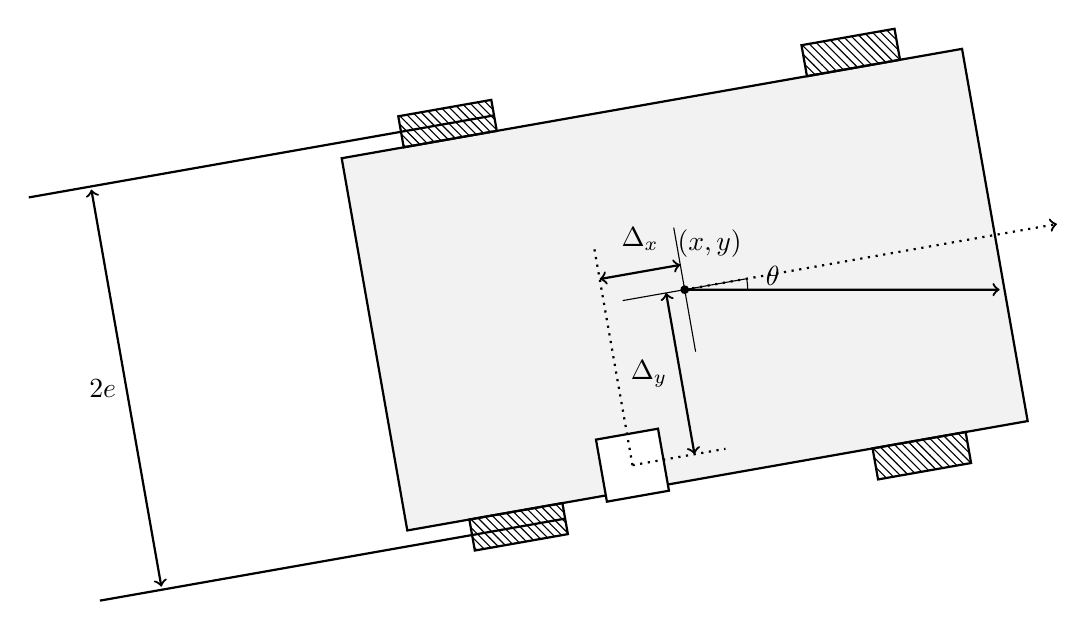
\begin{tikzpicture}[scale=0.8,rotate=-80]
		
	%Base
	\draw[thick, draw=black, fill=gray!10] (0,0) rectangle (6,10);
	\coordinate (center) at (3,5);
	\fill (center) circle [radius=2pt] node [above, xshift=9, yshift=8] {$(x,y)$} ;
	\draw (3,4) -- (3,6);
	\draw (2,5) -- (4,5);

	%Wheels
	\draw[thick, pattern=north west lines, pattern color=black] (-.5,1) rectangle (0,2.5);
	\draw[thick, pattern=north west lines, pattern color=black] (-.5,7.5) 	rectangle (0,9);
	\draw[thick, pattern=north west lines, pattern color=black] (6,1) rectangle (6.5,2.5);
	\coordinate (d0) at (6.25, 5);
	\draw[thick, pattern=north west lines, pattern color=black] (6,7.5) rectangle (6.5,9);
	
	%Sensors
	%\draw[thick, draw=black, fill=white]	(-.1,.25) 		rectangle 	(.5,.75);
	%\draw[thick, draw=black, fill=white] 	(-.1,9.25) 		rectangle 	(.5,9.75);
	%\draw[thick, draw=black, fill=white] 	(5.5,.25) 		rectangle 	(6.1,.75);
	\draw[thick, draw=black, fill=white] 	(5.1,3.2) 	rectangle 	(6.1,4.2);
	\coordinate (sensor) at (5.6,3.7);
	%\draw[thick, draw=black, fill=white] 	(2.5,10.25) 	rectangle 	(3.5,9.5);
	
	%Wheelbase
	\draw[thick, draw=black] 	(-.25,2.5)  -- (-.25,-5);
	\draw[thick, draw=black] 	(6.25,2.5)  -- (6.25,-5);
	\draw[thick, draw=black, <->](-.2, -4) -- (3,-4) node[left] {$2e$} --(6.2,-4);
	
	%Speed vector
	\draw[thick, draw=black, dotted, ->] (center) --+ (90:6);
	\draw[thick, draw=black, ->] (center) --+ (80:5cm);
	\draw ($(center) + (0,1)$) arc (90:80:1) node[right, yshift=5, xshift=3]{$\theta$};
	
	%Dx and Dy
	\draw[thick, dotted] (sensor) --+ (90:1.5);
	\draw[thick, dotted] (sensor) --+ (180:3.5);
	\draw[thick, <->] ($(sensor) + (0,1)$) --+ (-2.6,0) node [midway, left, xshift=-1]{$\Delta_y$};
	\draw[thick, <->] ($(sensor) + (-3,0)$) --+ (0,1.3) node[midway, above, yshift=4]{$\Delta_x$};
	
	\end{tikzpicture}
	
\end{document}  